\documentclass[10pt,a4paper,spanish]{report}

\usepackage[spanish]{babel}
\usepackage[utf8]{inputenc}
\usepackage{amsmath, amsthm}
\usepackage{amsfonts, amssymb, latexsym}
\usepackage{enumerate}
\usepackage[official]{eurosym}
\usepackage{graphicx}
\usepackage[usenames, dvipsnames]{color}
\usepackage{colortbl}
\usepackage{multirow}
\usepackage{fancyhdr}
\usepackage[all]{xy}
\usepackage{pgfplots}
\usepackage{algpseudocode}
\usepackage{listings}
\usepackage{titlesec}

\pgfplotsset{compat=1.5}

% a4large.sty -- fill an A4 (210mm x 297mm) page
% Note: 1 inch = 25.4 mm = 72.27 pt
%       1 pt = 3.5 mm (approx)

% vertical page layout -- one inch margin top and bottom
\topmargin      0 mm    % top margin less 1 inch
\headheight     0 mm    % height of box containing the head
\headsep       10 mm    % space between the head and the body of the page
\textheight   250 mm
\footskip      14 mm    % distance from bottom of body to bottom of foot

% horizontal page layout -- one inch margin each side
%\oddsidemargin    0   mm    % inner margin less one inch on odd pages
%\evensidemargin   0   mm    % inner margin less one inch on even pages
%\textwidth      159.2 mm    % normal width of text on page

\usepackage[math]{iwona}
\usepackage[T1]{fontenc}
\usepackage{inconsolata}

\usepackage[pdftex, bookmarks=true,
	bookmarksnumbered=false, % true means bookmarks in
	% left window are numbered
	bookmarksopen=false,     % true means only level 1
	% are displayed.
	colorlinks=true,
linkcolor=webblue]{hyperref}

\definecolor{webgreen}{rgb}{0, 0.5, 0} % less intense green
\definecolor{webblue}{rgb}{0, 0, 0.5}  % less intense blue
\definecolor{webred}{rgb}{0.5, 0, 0}   % less intense red
\definecolor{dblackcolor}{rgb}{0.0,0.0,0.0}
\definecolor{dbluecolor}{rgb}{.01,.02,0.7}
\definecolor{dredcolor}{rgb}{0.8,0,0}
\definecolor{dgraycolor}{rgb}{0.30,0.3,0.30}

\newcommand{\HRule}{\rule{\linewidth}{0.5mm}} % regla horizontal para  el titulo

\pagestyle{fancy}
%con esto nos aseguramos de que las cabeceras de capítulo y de sección vayan en minúsculas

\renewcommand{\chaptermark}[1]{%
	\markboth{#1}{}}
\renewcommand{\sectionmark}[1]{%
	\markright{\thesection\ #1}}
\fancyhf{} %borra cabecera y pie actuales
\fancyhead[LREO]{\bfseries\thepage}
\fancyhead[LO]{\bfseries\leftmark}
\renewcommand{\headrulewidth}{0.5pt}
\renewcommand{\footrulewidth}{0pt}
\addtolength{\headheight}{0.5pt} %espacio para la raya
\fancypagestyle{plain}{%
	\fancyhead{} %elimina cabeceras en páginas "plain"
	\renewcommand{\headrulewidth}{0pt} %así como la raya
}

%%%%% Para cambiar el tipo de letra en el título de la sección %%%%%%%%%%%
\usepackage{sectsty}
\chapterfont{\fontfamily{pag}\selectfont} %% for chapter if you want
\sectionfont{\fontfamily{pag}\selectfont}
\subsectionfont{\fontfamily{pag}\selectfont}
\subsubsectionfont{\fontfamily{pag}\selectfont}
\titleformat{\chapter}{\normalfont\Huge}{}{0pt}{\Huge} % Capítulos sin "Capítulo x" encima del título

\renewcommand{\labelenumi}{\arabic{enumi}. }
\renewcommand{\labelenumii}{\labelenumi\alph{enumii}) }
\renewcommand{\labelenumiii}{\labelenumii\roman{enumiii}: }

\title{Seguridad y Protección de Sistemas Informáticos \\
Criptosistemas Asimétricos}
\author{David Sánchez Jiménez}

\begin{document}
\begin{titlepage}
 \begin{center}
  \HRule \\[0.8cm]
  \textsc{\huge Seguridad y Protección \\ de Sistemas Informáticos \\[0.5cm] Criptosistemas Asimétricos}\\[1.6cm]
  \HRule \\[1cm]
  \begin{flushleft}
   \emph{Hecho por:}\\
   David Sánchez Jiménez
  \end{flushleft}
  \vspace{12cm}
  \large{\today}\\
  \vspace{0.5cm}
  \htmladdnormallink{
\includegraphics[width=2cm]{Imagenes/88x31.png}}
  {http://creativecommons.org/licenses/by-nc/4.0/}\\[0.5cm]
  \texttt{Prácticas de Seguridad y Protección de Sistemas Informáticos\\ by
   \href{mailto:dasaji92@gmail.com}{David Sánchez Jiménez} is licensed under a \htmladdnormallink{Creative Commons Reconocimiento-NoComercial-CompartirIgual 4.0 Internacional License}
   {http://creativecommons.org/licenses/by-nc/4.0/}}.\\[3mm]
 \end{center}
\end{titlepage}

\tableofcontents
\newpage

% ----------------------------------------------------------------
\chapter{Ejercicio 1}

\section{Enunciado}
\noindent
Generad, cada uno de vosotros, una clave RSA (que contiene el par de claves) de 768 bits. Para referirnos a ella supondré que se llama nombreRSAkey.pem. Esta clave no es necesario que esté protegida por contraseña.

\section{Respuesta}
\noindent
Generamos el archivo davidRSAkey.pem que almacene una clave RSA de 768 bits y mostramos el archivo por pantalla de la siguente manera:

\begin{figure}[!hbp]
 \centering  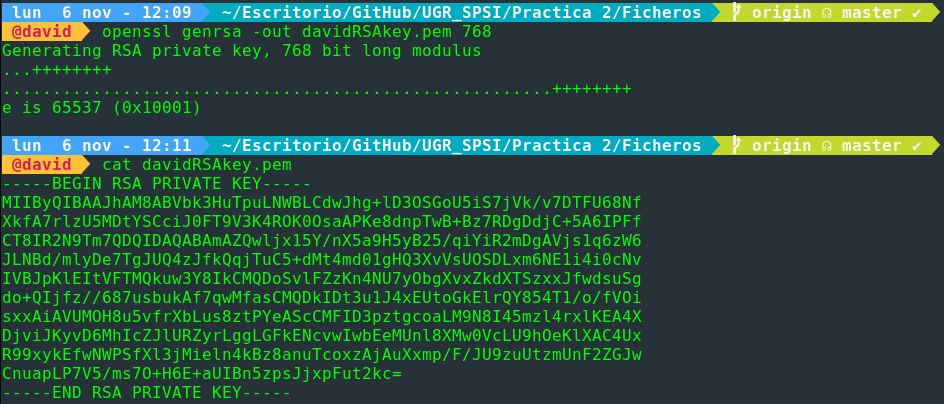
\includegraphics[width=1\textwidth]{./Imagenes/1.png}
\end{figure}


% ----------------------------------------------------------------
\chapter{Ejercicio 2}

\section{Enunciado}
\noindent
Extraed la clave provada contenida en el archivo nombreRSAkey.pem a otro archivo que tenga por nombre nombreRSApriv.pem. Este archivo deberá estar protegido por contraseña cifrándolo con AES-128. Mostrad sus valores.

\section{Respuesta}
\noindent
Para extraer la clave privada del archivo davidRSAkey.pem en el archivo davidRSApriv.pem utilizaremos las siguientes opciones:

\begin{itemize}
 \item Con el modificador -aes128 ciframos el fichero de salida, utilizaremos como contraseña 0123456789.
 \item Con el modificador -in indicamos el fichero del que se va a extraer la clave privada.
 \item Con el modificador -out indicamos el fichero de salida en el que almacenaremos la clave privada.
\end{itemize}

\noindent
El comando completo para extraer la clave privada sería el siguiente:

\begin{figure}[!hbp]
 \centering  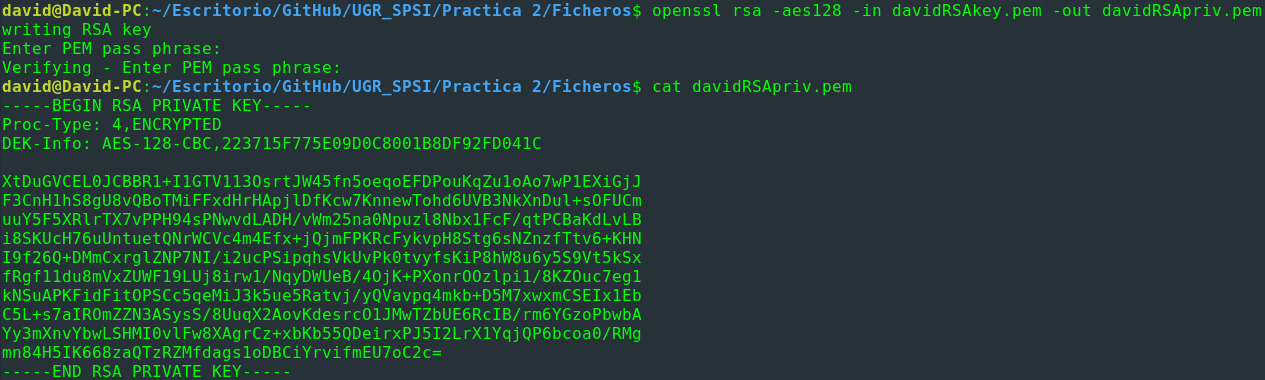
\includegraphics[width=1\textwidth]{./Imagenes/2_0.png}
\end{figure}

\newpage
\noindent
Ahora muestro el contenido del fichero de salida:

\begin{figure}[!hbp]
 \centering  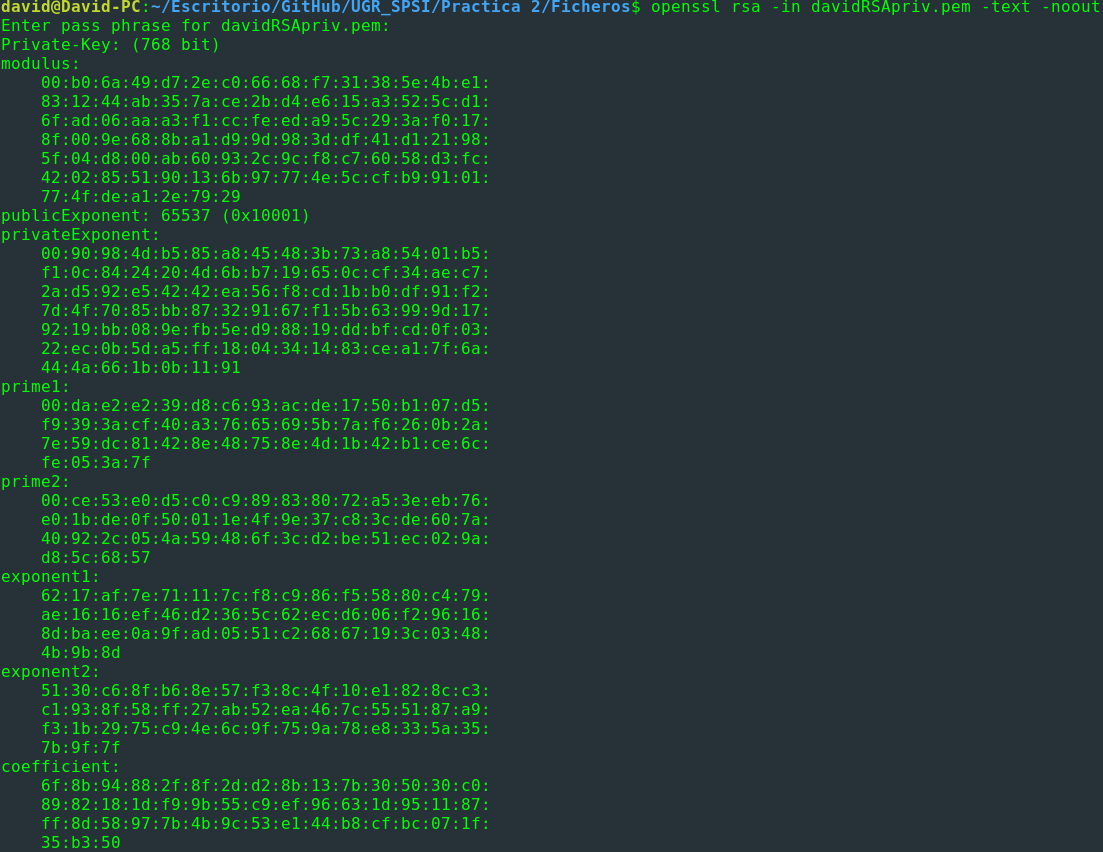
\includegraphics[width=1\textwidth]{./Imagenes/2_1.png}
\end{figure}

% ----------------------------------------------------------------
\chapter{Ejercicio 3}

\section{Enunciado}
\noindent
Extraed en nombreRSApub.pem la clave pública contenida en el archivo nombreRESAkey.pem. Evidentemente nombreRSApub.pem no debe estar cifrado ni protegido. Mostrad sus valores.

\section{Respuesta}
\noindent
Para extraer la clave privada del archivo davidRSAkey.pem en el archivo davidRSApriv.pem utilizaremos las siguientes opciones:

\begin{itemize}
 \item Con el modificador -pubout indicamos que queremos extraer la clave pública.
 \item Con el modificador -in indicamos el fichero del que se va a extraer la clave pública.
 \item Con el modificador -out indicamos el fichero de salida en el que almacenaremos la clave pública.
\end{itemize}

\noindent
El comando completo para extraer la clave pública sería el siguiente:

\begin{figure}[!hbp]
 \centering  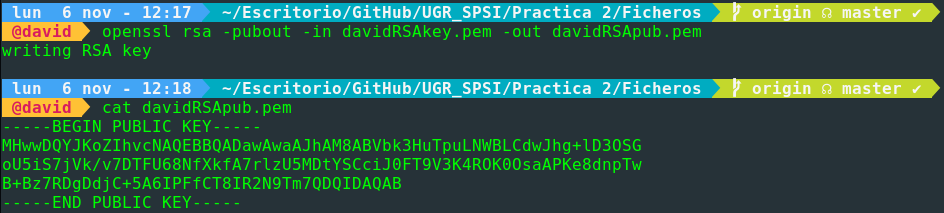
\includegraphics[width=1\textwidth]{./Imagenes/3_0.png}
\end{figure}

\noindent
Ahora muestro el contenido del fichero de salida:

\begin{figure}[!hbp]
 \centering  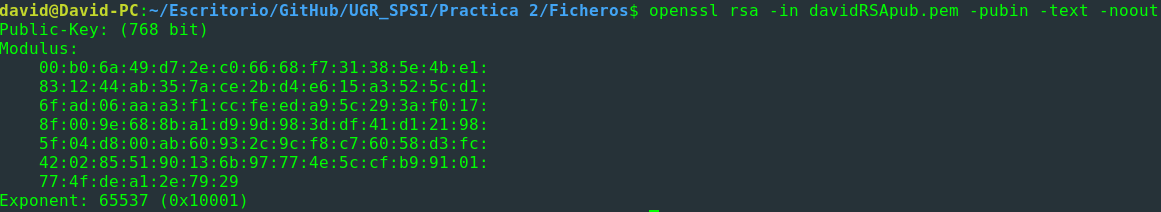
\includegraphics[width=1\textwidth]{./Imagenes/3_1.png}
\end{figure}


% ----------------------------------------------------------------
\chapter{Ejercicio 4}

\section{Enunciado}
\noindent
Reutilizaremos el archivo binario input.bin de 1024 bits, todos ellos con valor 0, de la practica anterior.

\section{Respuesta}
\noindent
Utilizaré el fichero input.bin de la anterior práctica. Su contenido es el siguiente:

\begin{figure}[!hbp]
 \centering  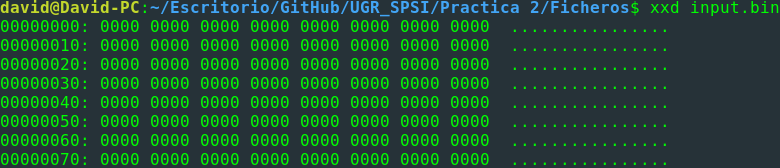
\includegraphics[width=1\textwidth]{./Imagenes/4.png}
\end{figure}

% ----------------------------------------------------------------
\chapter{Ejercicio 5}

\section{Enunciado}
\noindent
Intentad cifrar input.bin con vuestras claves pública. Explicad el resultado.

\section{Respuesta}
\noindent
Al intentar cifrar el archivo input.bin utilizando la clave pública generada en anteriormente obtenemos un error debido a que el fichero es de 1024 bits y la clave publica es de 768 bits, por lo que al ser el mensaje mayor que la clave no puede cifrarse.

\begin{figure}[!hbp]
 \centering  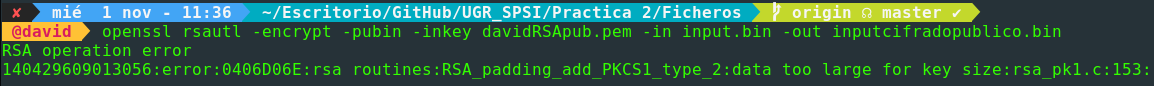
\includegraphics[width=1\textwidth]{./Imagenes/5.png}
\end{figure}

% ----------------------------------------------------------------
\chapter{Ejercicio 6}

\section{Enunciado}
\noindent
Diseñad un cifrado híbrido, con RSA como criptosistema asimétrico. El modo de proceder será el siguiente:
\begin{enumerate}
 \item El emisor debe seleccionar un sistema simétrico con su correspondiente modo de operación.
 \item El emisor generará un archivo de texto, llamado por ejemplo sessionkey con dos líneas. La primera línea contendrá una cadena aleatoria hexadecimal cuya longitud sea la requerida por la clave. OpenSSL permite generar cadenas aleatorias con el comando openssl rand. La segunda línea contendrá la información del criptosistema simétrico seleccionado. Por ejemplo, si hemos decidido emplear el algoritmo Blowfish en modo ECB la segunda línea debería contener -bf-ecb.
 \item El archivo sessionkey se cifrará con la clave pública del receptor.
 \item El mensaje se cifrará utilizando el criptosistema simétrico, la clave se generará a partir del archivo anterior mediante la opción -pass file:sessionkey.
\end{enumerate}

\section{Respuesta}
\noindent

% ----------------------------------------------------------------
\chapter{Ejercicio 7}

\section{Enunciado}
\noindent
Utilizando el criptosistema híbrido diseñado, cada uno debe cifrar el archivo input.bin con su clave pública para, a continuación descifrarlo con la clave privada. Comparad el resultado con el archivo original.

\section{Respuesta}
\noindent

% ----------------------------------------------------------------
\chapter{Ejercicio 8}

\section{Enunciado}
\noindent
Generad un archivo stdECparam.pem que contenga los parámetros públicos de una de las curvas elípticas contenidas en las transparencias de teoría. Si no lográis localizarlas haced el resto de la práctica con una curva cualquiera a vuestra elección de las disponibles en OpenSSL. Mostrad los valores.

\section{Respuesta}
\noindent

% ----------------------------------------------------------------
\chapter{Ejercicio 9}

\section{Enunciado}
\noindent
Generad cada uno de vosotros una clave para los parámetros anteriores. La clave se almacenará en nombreECkey.pem y no es necesario protegerla con contraseña.

\section{Respuesta}
\noindent

% ----------------------------------------------------------------
\chapter{Ejercicio 10}

\section{Enunciado}
\noindent
Extraed la clave privada contenida en el archivo nombreECkey.pem a otro archivo que tenga por nombre nombreECpriv.pem. Este archivo deberá estar protegido por contraseña cifrándolo con 3DES. Mostrad sus valores.

\section{Respuesta}
\noindent


% ----------------------------------------------------------------
\chapter{Ejercicio 11}

\section{Enunciado}
\noindent
Extraed en nombreECpub.pem la clave pública contenida en el archivo nombreECkey.pem. Como antes nombreECpub.pem no debe estar cifrado ni protegido. Mostrad sus valores.

\section{Respuesta}
\noindent

% ----------------------------------------------------------------
\end{document}
